\documentclass[tikz,border=2pt]{standalone}
\usepackage{amsmath}
\usepackage{pgfplots}
\pgfplotsset{compat=1.18}

\begin{document}
% The characteristic polynomial of A = [[2,1],[1,2]] is p(lambda) = (2-lambda)^2 - 1
% = lambda^2 - 4 lambda + 3; its roots 1 and 3 are the eigenvalues of A.
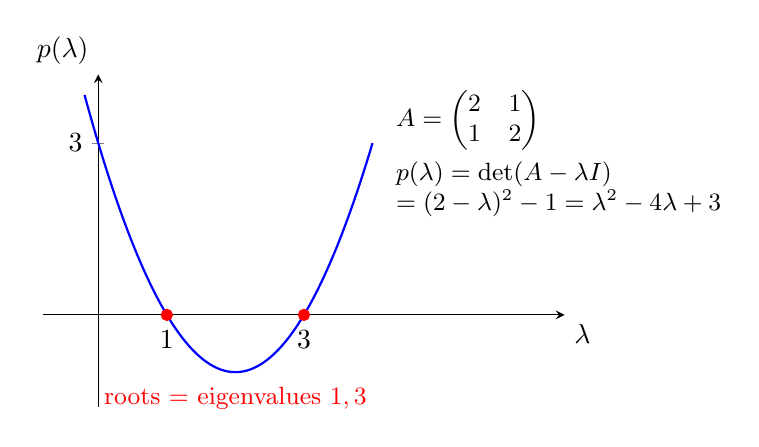
\begin{tikzpicture}
	\begin{axis}[
		axis lines=middle,
		xmin=-0.8, xmax=6.8, ymin=-1.6, ymax=4.2,
		xtick={1,3}, ytick={3},
		xlabel={$\lambda$}, ylabel={$p(\lambda)$},
		xlabel style={below right}, ylabel style={above left},
		samples=120, smooth, clip=false,
		width=8.2cm, height=5.8cm
		]
		\addplot[thick, blue, domain=-0.2:4.0] {x^2-4*x+3};
		\addplot[only marks, mark=*, red, mark size=2pt] coordinates {(1,0) (3,0)};
		\node[red, anchor=north, font=\small] at (axis cs:2,-1.1) {roots $=$ eigenvalues $1,3$};
		\node[anchor=north west, font=\small, align=left] at (axis cs:4.2,4.1) {$A=\begin{pmatrix}2&1\\1&2\end{pmatrix}$\\[3pt] $p(\lambda)=\det(A-\lambda I)$\\ $=(2-\lambda)^2-1=\lambda^2-4\lambda+3$};
	\end{axis}
\end{tikzpicture}
\end{document}
